%%%%%%%%%%%%%%%%%%%%%%%%%%%%%%%%%%%%%%%%%%%%%%%%%%%%%%%%%%%%%%%%%%%%%%%%%%%%%%%%%%%%%%%%%%%%%%%%%%%%%%%%%%%%%%%%%%%%%%%%<

% 12, 14, 17, 20, 25
\documentclass[a0paper, portrait, 25pt,
margin=0mm, innermargin=15mm, blockverticalspace=15mm, colspace=15mm, subcolspace=8mm
]{tikzposter}

%%%%%%%%%%%%%%%%%%%%%%%%%%%%%%%%%%%%%%%%%%%%%%%%%%%%%%%%%%%%%%%%%%%%%%%%%%%%%%%%%%%%%%%%%%%%%%%%%%%%%%%%%%%%%%%%%%%%%%%%<

\usepackage{iftex}

%**** Encoding and Font **************************

\ifPDFTeX
  \usepackage[utf8]{inputenc}
  \usepackage[T1]{fontenc}
  \usepackage{lmodern} % Postscript layout of CM with T1 coding
\else
  \ifLuaTeX
    \usepackage[T1]{fontenc}
    \usepackage{lmodern} % Postscript layout of CM with T1 coding
    \hypersetup{pdfencoding=auto}
  \fi
\fi

%**** Language ***********************************

% \usepackage[frenchb]{babel}
%\usepackage[english]{babel}
% \usepackage{frenchle} % compatibility?

%%%%%%%%%%%%%%%%%%%%%%%%%%%%%%%%%%%%%%%%%%%%%%%%%%%%%%%%%%%%%%%%%%%%%%%%%%%%%%%%%%%%%%%%%%%%%%%%%%%%%%%%%%%%%%%%%%%%%%%%<

\title{Une interface expérimentale pour lier OpenGL à Python}
\author{Fabrice~Salvaire}
% \institute{}
\pgfdeclareimage[height=10cm]{FunnyPython}{images/funny-python.png}
\pgfdeclareimage[height=10cm]{OpenGLLogo}{images/OpenGL_1500.png}
\titlegraphic{\pgfuseimage{OpenGLLogo}\pgfuseimage{FunnyPython}}

\newcommand{\emailOrange}{fabrice.salvaire@orange.fr}
\newcommand{\homePageOrange}{\url{http://fabrice-salvaire.pagesperso-orange.fr}}
% \newcommand{\homePageGithub}{\url{http://fabricesalvaire.github.io}}
\newcommand{\githubRepositories}{\url{http://github.com/FabriceSalvaire}}

% Theme:  Default, Basic, Rays, Simple, Envelope, Wave, Board, Autumn, Desert,
\usetheme{Board}
% \usecolorstyle[colorPalette=BrownBlueOrange]{Germany}

%%%%%%%%%%%%%%%%%%%%%%%%%%%%%%%%%%%%%%%%%%%%%%%%%%%%%%%%%%%%%%%%%%%%%%%%%%%%%%%%%%%%%%%%%%%%%%%%%%%%%%%%%%%%%%%%%%%%%%%%<

\begin{document}

\maketitle

\begin{columns}

% First column
\column{0.5}
\block{Architecture}{
  \begin{center}
  \begin{tikzpicture}[]
    %\draw[help lines] (-15,-20) grid (15,20);

    \node at (0,0) {\includegraphics[width=30cm]{images/tree.pdf}};
    \node at (-12,5) {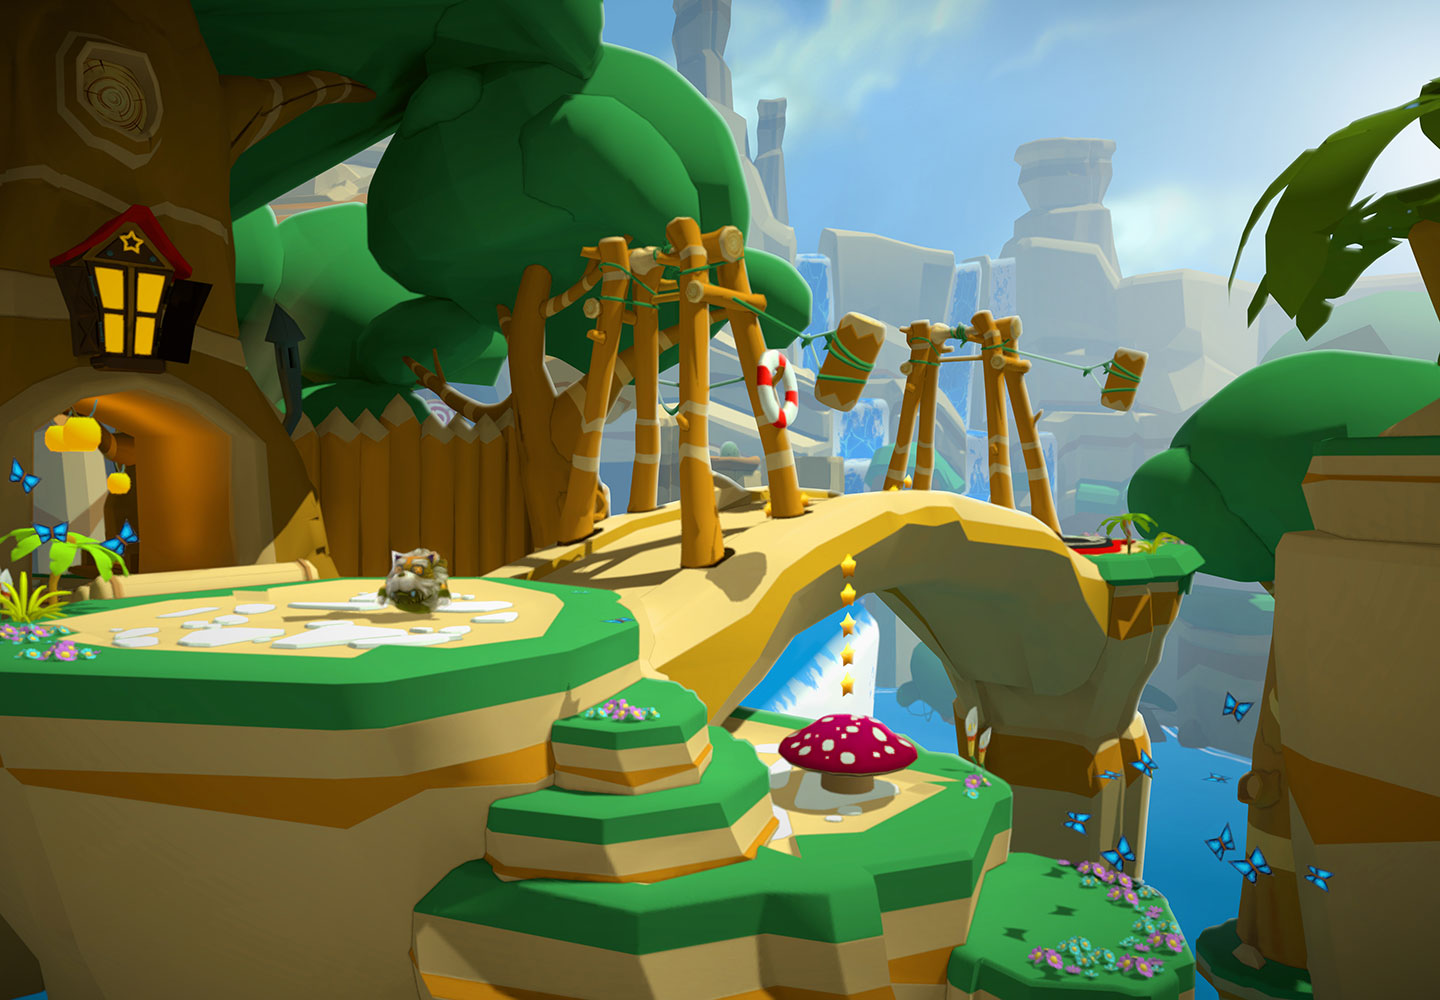
\includegraphics[width=10cm]{images/game.jpg}};
    \node at (-8,15) {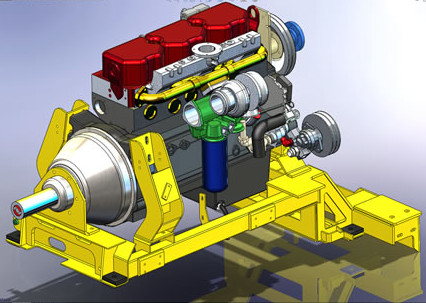
\includegraphics[width=10cm]{images/solidworks.jpg}};
    \node at (1,15) {
\includegraphics[height=10cm]{images/touchwiz.jpg}};
    \node at (8,10) {
\includegraphics[width=10cm]{images/tiger.png}};
    \node at (12,2) {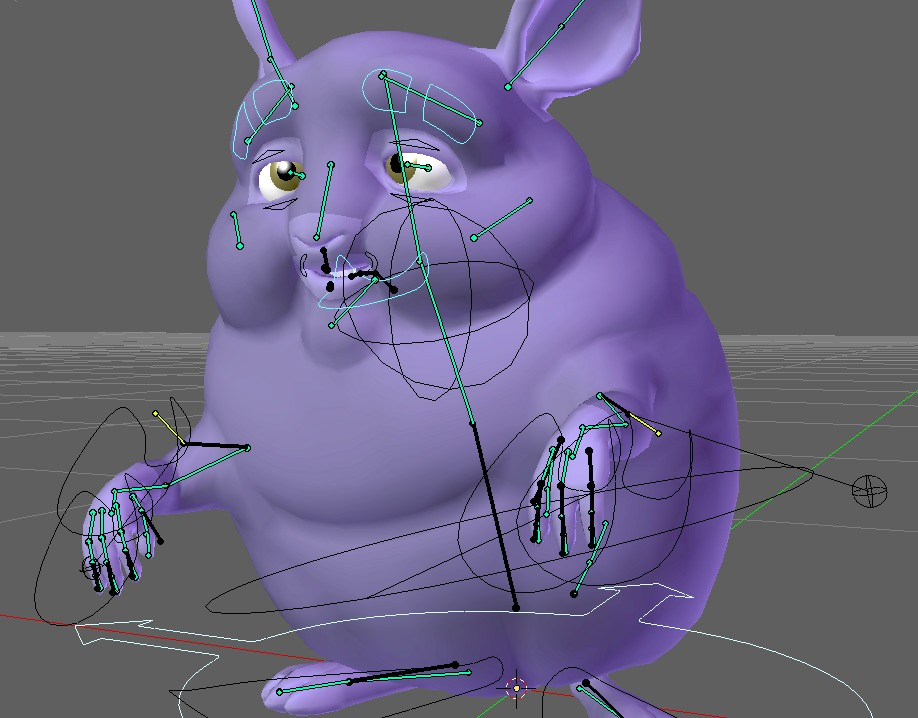
\includegraphics[width=8cm]{images/blender.jpg}};
    \node at (-14,-6) {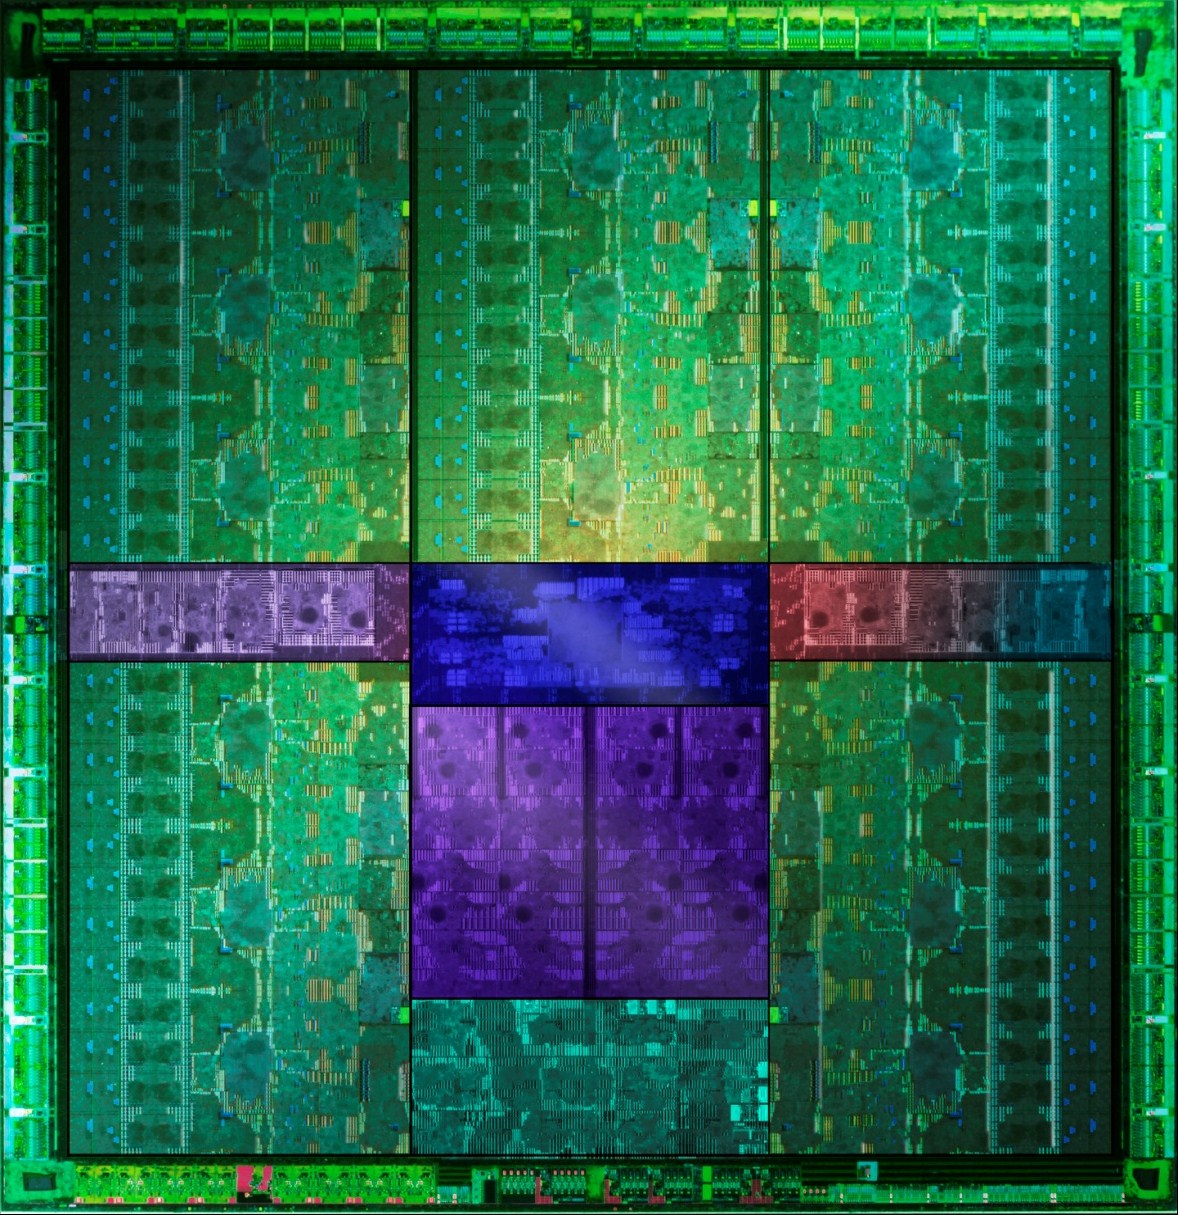
\includegraphics[width=6cm]{images/nvidia-kepler-die.jpg}};
    \begin{scope}[xshift=-3cm, yshift=-12cm,
      base/.style={rectangle, minimum width=10em, minimum height=2em, draw=white, line width=2pt,
        anchor=south west},
      double/.style={base, minimum height=4em},
      small/.style={base, minimum width=4em}]
      % \draw [help lines] grid(3,2);
      \node[base, fill=green!20] at (0,0) {XML Registry};
      \node[base, fill=red!20] at (0,2em) {GL API};
      \node[double, fill=blue!20] at (0,4em) {Wrapper};
      \node[small, fill=green!20] at (-4em,4em) {ctypes};
      \node[small, fill=red!20] at (-4em,6em) {cffi};
      \node[double, minimum width=4em, fill=blue!20] at (-8em,4em) {GL};
      \node[base, fill=green!20] at (0,8em) {High Level API};
    \end{scope}
    \end{tikzpicture}
  \end{center}
}

 % Second column
\column{0.5}

 % Second column - first block
\block[]{Foo}{Test}

\block[titleleft]{Contact: \emailOrange}{%
% \homePageOrange
  
\includegraphics[width=10cm]{figures/vcard.pdf} % check data
}

\end{columns}
\end{document}
\endinput

%%%%%%%%%%%%%%%%%%%%%%%%%%%%%%%%%%%%%%%%%%%%%%%%%%%%%%%%%%%%%%%%%%%%%%%%%%%%%%%%%%%%%%%%%%%%%%%%%%%%%%%%%%%%%%%%%%%%%%%%
%%%
%%% Local Variables: 
%%% mode: latex
%%% TeX-master: t
%%% End: 
%%%
%%%%%%%%%%%%%%%%%%%%%%%%%%%%%%%%%%%%%%%%%%%%%%%%%%%%%%%%%%%%%%%%%%%%%%%%%%%%%%%%%%%%%%%%%%%%%%%%%%%%%%%%%%%%%%%%%%%%%%%%
